\chapter{双图决策树多端口构造条件证明}
\label{app:mpcon}

这里给出定理\ref{thm:mpcon}的解析方法证明,节\ref{sec:mp}已经从生成树对枚举的角度说明了定理的正确性。
这里将从解析表达式的角度给出证明。为方便起见,同样这里只给出了相应的条件a的证明过程。

考虑如图\ref{fig:provempcir}中的多端口电路,其中在电路左侧共有$n$个输入端口,以$w_1$至$w_n$标记,所有的输出均在右侧的端口观测信号$y$。

\begin{figure}[!htp]
	\centering
	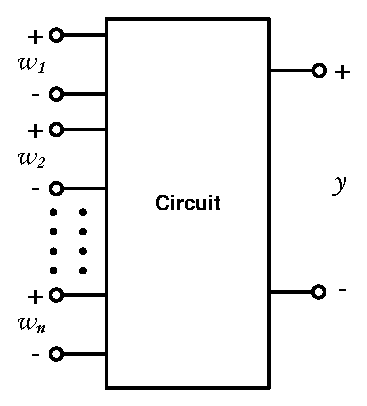
\includegraphics[width=0.3\textwidth]{app2/ProveMPCir.eps}
	\bicaption[fig:provempcir]{多端口电路构建条件证明示意电路图}{多端口电路构建条件证明示意电路图}{Fig}{Circuit for multi-port construction condition proof}
\end{figure}

假设图\ref{fig:provempcir}对应的GPDD结构在前$n$层结构如图\ref{fig:provempgpdd}所示,有着完整二叉树结构,故拥有从$T_{2^n-1}$至$T_0$个GPDD子结构。为了简化计算,这里所有的符号均假设为正号。

\begin{figure}[!htp]
	\centering
	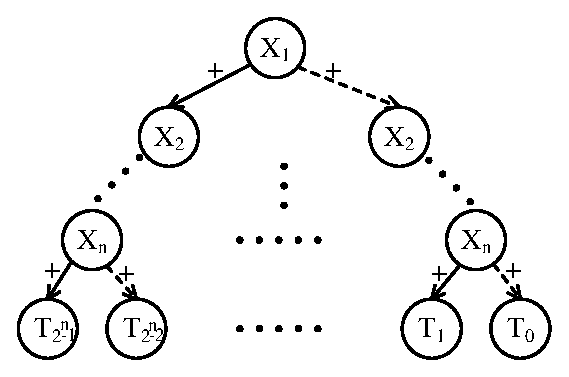
\includegraphics[width=0.6\textwidth]{app2/ProveMPGPDD.eps}
	\bicaption[fig:provempgpdd]{多端口电路构建条件证明示意初始GPDD结构}{多端口电路构建条件证明示意初始GPDD结构}{Fig}{Initial GPDD structure for Circuit for multi-port construction condition proof}
\end{figure}

结合两张图的结果,可以得到,某一对输入输出端口的电路传输函数应如下式所示。

\begin{equation}
{H_i} = {\left. {\frac{y}
		{{{w_i}}}} \right|_{{w_j} = 0,j \in [1,n]\backslash \{ i\} }} = \frac{1}
{{{X_i}}} =  - \frac{{{T_{{2^{n - i}}}}}}
{{{T_0}}},i \in [1,n]
\end{equation}

从图\ref{fig:provempgpdd}中可以看到,如果我们可以证明除去2的倍数的所有的$T_i$均为0,那么就不存在交叉的$X_i$和$X_j$。
为了接下来计算方便,我们引入记号$\beta_n\left(i,j\right)$,用来表示$i$的$n$位二进制表达中的第$n-j+1$位。由于GPDD整个结构求和等于零,可以得到如下推导关系:

\begin{align}
&\sum\limits_{i = 0}^{{2^n} - 1} {{T_i}\prod\limits_{j = 1}^n {X_j^{{\beta _n}\left( {i,j} \right)}} }  = 0\\
&{T_0} + \sum\limits_{i = 1}^n {{T_{{2^{n - i}}}}{X_i}}  + \sum\limits_{i \in \left[ {1,{2^n} - 1} \right]\backslash \left\{ {\left. {{2^{n - i}}} \right|i \in \left[ {1,n} \right]} \right\}} {{T_i}\prod\limits_{j = 1}^n {X_j^{{\beta _n}\left( {i,j} \right)}} }  = 0\\
&{T_0} + \sum\limits_{i = 1}^n {{T_{{2^{n - i}}}}{X_i}}  + R = 0\\
&1 + \sum\limits_{i = 1}^n {\frac{{{T_{{2^{n - i}}}}}}{{{T_0}}}{X_i}}  + \frac{1}{{{T_0}}}R = 0\\
&1 - \sum\limits_{i = 1}^n {{H_i}{X_i}}  + \frac{1}{{{T_0}}}R = 0\\
&y - \sum\limits_{i = 1}^n {y{H_i}{X_i}}  + \frac{y}{{{T_0}}}R = 0\\
&y - \sum\limits_{i = 1}^n {{w_i}{H_i}}  + \frac{y}{{{T_0}}}R = 0
\end{align}

其中用到剩余项$R$来简化推导过程,$R$则等于:

\begin{equation}\label{eq:remain}
R=\sum\limits_{i \in \left[ {1,{2^n} - 1} \right]\backslash \left\{ {\left. {{2^{n - i}}} \right|i \in \left[ {1,n} \right]} \right\}} {{T_i}\prod\limits_{j = 1}^n {X_j^{{\beta _n}\left( {i,j} \right)}} }
\end{equation}

根据电路的叠加定理,可以有:
\begin{equation}
y = \sum\limits_{i = 1}^n {{H_i}{w_i}}
\end{equation}

结合前面的推导可以知道推导的剩余部分$R$为0,即:

\begin{equation}
\frac{y}{{{T_0}}}R = 0 \Rightarrow R=0
\end{equation}

我们知道在式\ref{eq:remain}中,所有的$X_i$均为未知量,要使恒等式成立,那么当且仅当此处所有的$T_i$为零,即:

\begin{equation}
{T_i} = 0,i \in \left[ {1,{2^n} - 1} \right]\backslash \left\{ {\left. {{2^{n - i}}} \right|i \in \left[ {1,n} \right]} \right\}
\end{equation}

所以,所有非2的倍数序号的GPDD子结构均为零,根据GPDD的约减规则,自然会得到如图\ref{fig:proveres}所示的简化GPDD结构。

\begin{figure}[!htp]
	\centering
	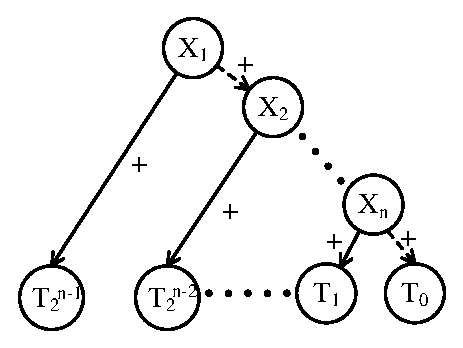
\includegraphics[width=0.4\textwidth]{app2/ProveRes.eps}
	\bicaption[fig:proveres]{多端口电路构建条件证明示意最终GPDD结构}{多端口电路构建条件证明示意最终GPDD结构}{Fig}{Final GPDD structure for Circuit for multi-port construction condition proof}
\end{figure}